% ECE 253 project report, ICASSP 2027 template (spconf.sty, IEEEbib.bst).  Build: cd report && latexmk -pdf paper.tex
% Tables (tables/*.tex) and figures (figures/*.pdf) are generated: src/report/make_tables.py, src/report/make_figures.py.
\documentclass{article}
\usepackage{spconf,amsmath,amssymb,graphicx,booktabs,hyperref}
\hypersetup{hidelinks}
\setlength{\tabcolsep}{3.2pt}
\setlength{\textfloatsep}{8pt plus 2pt minus 2pt}
\setlength{\dbltextfloatsep}{8pt plus 2pt minus 2pt}
\setlength{\floatsep}{6pt plus 2pt minus 2pt}
\setlength{\dblfloatsep}{6pt plus 2pt minus 2pt}
\setlength{\abovecaptionskip}{3pt}\setlength{\belowcaptionskip}{3pt}

\setcounter{topnumber}{4}\setcounter{dbltopnumber}{4}\setcounter{totalnumber}{6}
\renewcommand{\topfraction}{.95}\renewcommand{\dbltopfraction}{.95}\renewcommand{\textfraction}{.05}
\renewcommand{\floatpagefraction}{.9}\renewcommand{\dblfloatpagefraction}{.9}

\title{Improving ID Card Scanning and Recognition:\\Out-of-Focus Blur and Specular Highlight Removal}
\name{Aaryan Garg, Myles Lazarus}
\address{University of California, San Diego}

\begin{document}
\ninept
\maketitle

\begin{abstract}
Phone photos of identity cards suffer from out-of-focus blur and specular glare, which break optical character recognition (OCR). For each artifact we adapt one classical and one learned method, and test them alone and chained on 141 photos of 22 cards and on 200 external captures from MIDV-2020. We score OCR on fixed text boxes, per glare zone, with two engines and paired confidence intervals. A fine-tuned Restormer raises Tesseract accuracy on blurred test cards by 0.38; Wiener filtering does not transfer to unseen cards. Learned glare removal helps Tesseract but hurts PaddleOCR, on our cards and on MIDV-2020. Clipped text returns only with several frames: fusing a short clip raises its PaddleOCR accuracy from 0.48 to 0.99. With both artifacts, deblurring does most of the work and the order makes no significant difference. SSIM and OCR often disagree.
\end{abstract}
\begin{keywords}
Defocus deblurring, specular highlight removal, document OCR, multi-frame fusion, identity documents
\end{keywords}

\section{Introduction}
\label{sec:intro}
Banks, airlines and web services read identity (ID) cards from phone photos. Two capture artifacts are common. \emph{Out-of-focus blur} merges neighboring characters. \emph{Specular glare} on the laminate has a \emph{core}, where the sensor clips and the text is gone, and a surrounding \emph{halo}, where text survives under a bright veil. Both cause wrong or missing fields. Restoration can help, but a network that invents strokes is dangerous when the output is a date or an ID number.

We ask whether restoration makes cards more readable, and for which reader. For each artifact we take a classical and a learned method, modify both for our data, and compare them with the unmodified versions and with no treatment. Our contributions are: (i) a paired dataset of 141 photos with blur, glare and both; (ii) an OCR protocol with fixed boxes, two engines and paired statistics, which removes text-detector noise; (iii) a classical veil estimator that needs no reference, and a highlight network with a detection head, designed to change only the glare; (iv) a replication of the glare results on 100 external photos, and multi-frame fusion on 100 clips; and (v) a study of chaining and its order.

\begin{figure*}[t]
\centering
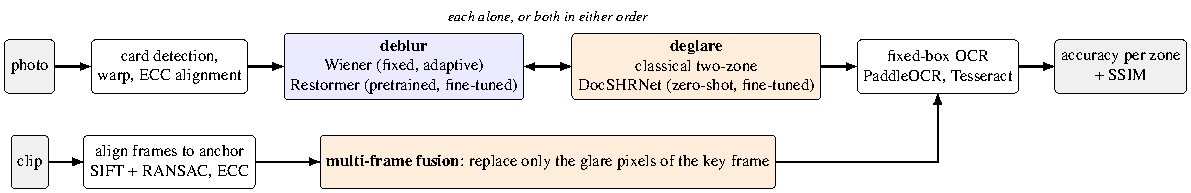
\includegraphics[width=\textwidth]{figures/pipeline}
\caption{The evaluated system. Single photos are deblurred, deglared, or both in either order. Clips are fused instead.}
\label{fig:pipeline}
\end{figure*}

\section{Relation to prior work}
\label{sec:prior}
\textbf{Blur.} Defocus is modeled as convolution with a disk. The Wiener filter~\cite{wiener1949} is its standard linear inverse; text-specific priors~\cite{cho2012} and CNNs for text~\cite{hradis2015} exploit the structure of characters. Defocus networks were driven by dual-pixel data~\cite{abuolaim2020} and adaptive filters~\cite{lee2021}; Restormer~\cite{zamir2022} and NAFNet~\cite{chen2022} are efficient general restorers.
\textbf{Glare.} The dichromatic model~\cite{shafer1985} separates diffuse and specular reflection~\cite{shen2013}. Clipped areas are usually inpainted~\cite{telea2004}, which also overwrites text that is still visible in the halo. Learned methods use paired data of objects~\cite{fu2021,wu2021} or documents~\cite{hou2021,leong2024,xu2025}. SHDocs~\cite{leong2024} also scores highlight removal by OCR.
\textbf{ID documents.} MIDV-500, MIDV-2019 and MIDV-2020~\cite{arlazarov2019,bulatov2020,bulatov2022} provide mock documents. Video recognition usually selects a frame~\cite{aliev2021} or combines per-frame readings.

Unlike these works we (a) treat both artifacts on the same cards and chain the methods, (b) report per glare zone, so that recoverable and lost text are not mixed, (c) test two OCR engines with paired intervals, and (d) compare single-image removal with fusion of pixels over frames.

\section{Data and evaluation}
\label{sec:data}
\begin{table*}[t]
\centering
\caption{Deblurring, test B ($n=4$ images, 54 boxes). Change: mean paired difference to untreated [95\% CI]; bold: the CI excludes 0 (changes) or best in column (accuracy). With $n=4$ the intervals are only rough.}
\label{tab:blur}
\begin{tabular}{lrlrll}
\toprule
 & \multicolumn{2}{c}{PaddleOCR} & \multicolumn{2}{c}{Tesseract} & \multicolumn{1}{c}{SSIM} \\
\cmidrule(lr){2-3}\cmidrule(lr){4-5}\cmidrule(lr){6-6}
method & acc. & change [95\% CI] & acc. & change [95\% CI] & change [95\% CI] \\
\midrule
untreated & .782 & -- & .307 & -- & -- \\
Wiener, fixed & .568 & $-$.210 [$-$.566, .019] & .284 & $-$.084 [$-$.272, .103] & $-$.042 [$-$.115, .014] \\
Wiener, adaptive & .530 & $-$.236 [$-$.571, .019] & .242 & $-$.070 [$-$.229, .050] & $-$.012 [$-$.054, .017] \\
Restormer, pretrained & .809 & +.011 [$-$.030, .069] & .388 & \textbf{+.071 [.000, .126]} & \textbf{+.025 [.017, .034]} \\
Restormer, fine-tuned & \textbf{.838} & +.026 [$-$.103, .150] & \textbf{.745} & \textbf{+.376 [.233, .510]} & \textbf{+.074 [.040, .100]} \\
\midrule
reference & .989 & -- & .846 & -- & -- \\
\bottomrule
\end{tabular}

\end{table*}

\begin{figure}[t]
\centering
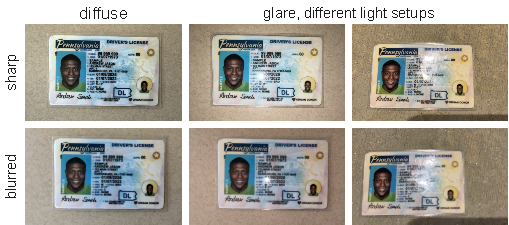
\includegraphics[width=\columnwidth]{figures/dataset}
\caption{One specimen card: sharp and blurred, diffuse light and glare.}
\label{fig:dataset}
\end{figure}

\textbf{Our data.} We photographed 22 card sides (14 fronts, 8 backs; 14 are real cards and 8 are printed, laminated specimens; only specimens are shown here) sharp and blurred, under diffuse light and under glare from different light setups (Fig.~\ref{fig:dataset}): 22 sharp references, 24 blurred, 47 glare, and 48 blur + glare photos (47 usable). Photos were taken hand-held, mostly with an iPhone 17 and some with an iPhone 12 Pro. Blur is real defocus: we focused on another object, locked the autofocus, and then photographed the card. The text of every card was typed by hand. Cards, not images, are split 14 / 4 / 4 into train / val / test. Test cards are never used for training or tuning in any condition; the test set has 4 blur (B), 8 glare (G) and 9 blur + glare (BG) images.

\textbf{Rectification.} Canny, color and GrabCut~\cite{rother2004} hypotheses vote for the card outline. The card is warped to $1012\times638$ px, and every photo is aligned to the card's reference with an ECC homography~\cite{evangelidis2008}, glare masked out, in a single interpolation.

\textbf{External data.} From MIDV-2020~\cite{bulatov2022} we use all captures labeled ``highlight present'': 100 photos and 100 clips of 200 documents (10 types). The flatbed scan is the reference. Nothing is trained or tuned on MIDV.

\textbf{Fixed-box OCR.} Whole-card OCR mixes restoration effects with text-detector noise. We therefore detect line boxes once, on the reference (on MIDV: the annotated fields), and only run \emph{recognition} on the same boxes in every version of an image: PaddleOCR (PP-OCRv6)~\cite{zhang2026} and Tesseract~\cite{smith2007} in single-line mode. Of 368 boxes on our cards, 342 get a label from the typed text. A box belongs to the \emph{core} (clipped, all channels $\ge248$), the \emph{halo} ($>40$ gray levels brighter than the reference), or \emph{outside}. The score is character accuracy, one minus the edit distance over the target length (letters and digits, case ignored), pooled over the boxes of a zone. Changes are mean paired differences per image with 95\% bootstrap intervals over images; $n$ is the number of images with a box in the zone. Re-reading the reference with 2-px shifts, noise and JPEG moves PaddleOCR by at most 0.006 per zone and Tesseract by up to 0.07. SSIM~\cite{wang2004} to the reference is secondary.

\section{Methods}
\label{sec:methods}
\begin{figure*}[t]
\centering
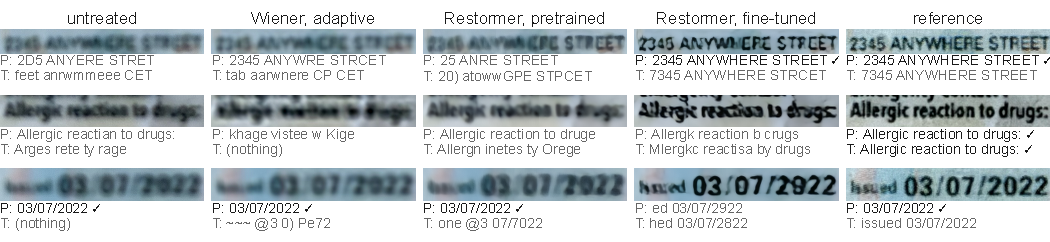
\includegraphics[width=\textwidth]{figures/blur_crops_small}
\caption{Deblurring of test lines with PaddleOCR (P) and Tesseract (T) readings; $\checkmark$: every letter and digit correct. Chosen to show a gain (top) and failures: in the last row the fine-tuned Restormer changes a correctly read year.}
\label{fig:blur}
\end{figure*}

All parameters were chosen on train and val, then frozen. Glare settings had to keep SSIM outside the glare within 0.002 of the untreated image (``do no harm''). Deblurring settings had to improve both accuracy and SSIM.

\subsection{Deblurring}
\textbf{Wiener.} With a disk PSF $H$ of radius $r$, we filter the luminance, $\hat F = H^*G/(|H|^2+K)$, with tapered borders. The \emph{fixed} version uses one setting for all images ($r=6$, $K=0.03$, grid search on 20 images). Our \emph{adaptive} version estimates $K=\lambda\sigma_n^2/\sigma_f^2$ from the median absolute deviation of the finest Haar band, and picks $r\in\{0,\dots,8\}$ per image by Tesseract confidence plus weighted sharpness minus ringing.

\textbf{Restormer}~\cite{zamir2022}, pretrained for single-image defocus, is run on 512-px tiles. We \emph{fine-tune} it on the 16 blurred training photos (128-px patches, 75\% near text, $L_1$, AdamW, learning rate $10^{-5}$). The sharp target is tone-matched to the blurred input, so that the network does not learn exposure changes. Step 1000 of 2000 was selected on val.

\subsection{Glare removal}
\begin{table}[t]
\centering
\caption{Glare: character accuracy (P: PaddleOCR, T: Tesseract, DL: DocSHRNet). Core / halo boxes: ours 5 / 26, MIDV 49 / 434.}
\label{tab:glare}
\setlength{\tabcolsep}{2pt}
\begin{tabular}{lrrrrrrrr}
\toprule
 & \multicolumn{2}{c}{P, ours} & \multicolumn{2}{c}{P, MIDV} & \multicolumn{2}{c}{T, ours} & \multicolumn{2}{c}{T, MIDV} \\
\cmidrule(lr){2-3}\cmidrule(lr){4-5}\cmidrule(lr){6-7}\cmidrule(lr){8-9}
method & core & halo & core & halo & core & halo & core & halo \\
\midrule
untreated & .444 & \textbf{.869} & \textbf{.636} & \textbf{.830} & .133 & .417 & .218 & .334 \\
classical & .378 & .854 & .484 & .829 & .178 & .480 & .159 & .333 \\
DL, zero-shot & .400 & .714 & .467 & .735 & .222 & .574 & .237 & .435 \\
DL, fine-tuned & \textbf{.467} & .817 & .511 & .754 & \textbf{.244} & \textbf{.620} & \textbf{.281} & \textbf{.447} \\
\midrule
reference & .978 & .994 & 1.000 & .995 & .867 & .837 & .922 & .900 \\
\bottomrule
\end{tabular}

\end{table}

\begin{figure*}[t]
\centering
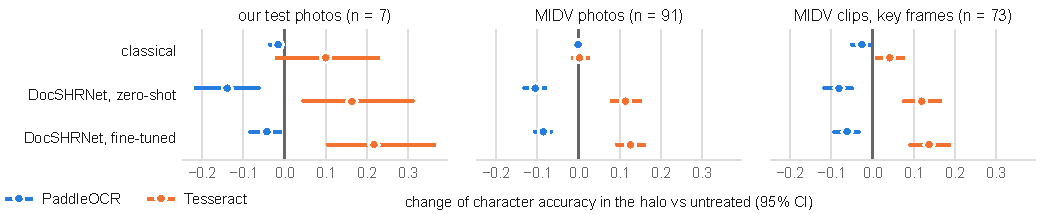
\includegraphics[width=\textwidth]{figures/halo_changes}
\caption{Single-image glare removal: paired change of halo accuracy. The networks' sign depends on the OCR engine.}
\label{fig:halo}
\end{figure*}

\textbf{Classical}. A fit of glare pixels against the reference (738 blocks) gives gain plus offset/255 of 0.96, which supports a white veil, $I=R(1-a)+255a$. Clipped blobs of at least 100 px are seeds; without seeds the image is returned unchanged. The old version assumed $a=a_0e^{-d/\tau}$ with the distance $d$ to the core. Our version measures the local black level $b$ of ink in textured blocks, similar in spirit to the dark channel prior~\cite{he2011}; interpolates the expected level $b_0$ from blocks far from the glare; and sets $a=(b-b_0)/(255-b_0)$, capped by the local white level. The veil is then inverted. Cores get a flat color instead of inpainting~\cite{telea2004}, which smeared strokes and made word F1 worse on 7 of 39 train and val images (better on 1).

\textbf{Learned}. The network planned first~\cite{fu2021} is no longer available. We use DocSHRNet~\cite{xu2025}, a NAFNet-style U-Net (34.6\,M parameters) pretrained on document highlights, and add a detection head $m$ on its last features. The output is $m\,y+(1-m)\,x$: pixels not detected as glare stay as they are. We fine-tune on 31 glare photos (256-px crops, 1500 iterations) with a glare-weighted $L_1$ loss, $0.2\,(1-\mathrm{SSIM})$, and $0.1$ times the cross-entropy of $m$ against the reference-derived glare mask.

\textbf{Fusion} of clips. Frames with at least 80\% of the document in view and no motion blur are aligned to one anchor (SIFT~\cite{lowe2004} + RANSAC, then ECC on locally normalized images with the glare masked) and kept if the residual is at most 1 px: 4641 of 6258 frames. A pixel is glare if it is clipped or $>30$ levels above its 25th percentile over time. \emph{Only glare pixels of the key frame are replaced}, by the mean of the frames where that pixel is clean. Baselines are the single frame and, per field, the frame with the least glare, and the temporal median. The key frame is the middle frame (\emph{keymid}) or the one with the most clipped text (\emph{keymax}).

\section{Results}
\label{sec:results}
\begin{figure*}[t]
\centering
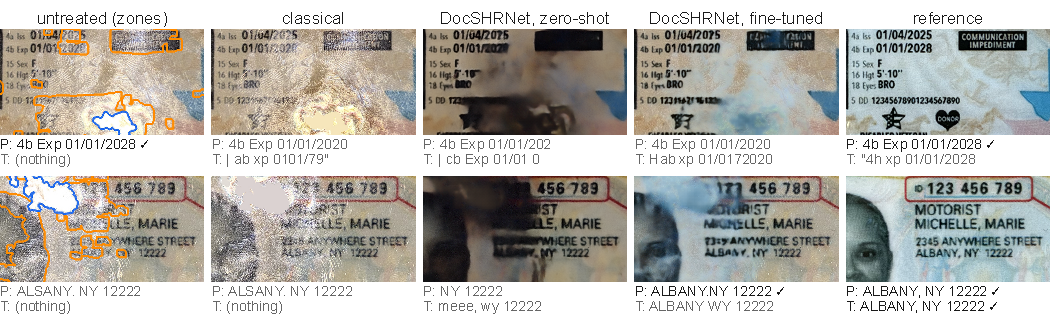
\includegraphics[width=\textwidth]{figures/glare_crops_small}
\caption{Glare removal on test cards (blue: core, orange: halo), with readings of the expiry date (top) and of the line ``ALBANY, NY 12222'' (bottom). Chosen to show harm (top, PaddleOCR) and gain (bottom).}
\label{fig:glare}
\end{figure*}


\subsection{Blur}
\begin{table*}[t]
\centering
\caption{Effect of each modification (new minus old version). B: all boxes; G: the named zone. SSIM: whole card (B), glare region (G). $n$: images with a box in the zone.}
\label{tab:mod}
\begin{tabular}{lllll}
\toprule
modification & test data (n) & PaddleOCR & Tesseract & SSIM \\
\midrule
Wiener: fixed $\rightarrow$ adaptive & B\_D (4) & $-$.026 [$-$.073, .000] & +.014 [$-$.084, .175] & \textbf{+.030 [.003, .057]} \\
Restormer: pretrained $\rightarrow$ fine-tuned & B\_D (4) & +.015 [$-$.073, .081] & \textbf{+.305 [.165, .412]} & \textbf{+.049 [.021, .071]} \\
classical: decay $\rightarrow$ statistics veil & S\_G, halo (7) & $-$.007 [$-$.018, .000] & \textbf{+.089 [.002, .252]} & +.009 [$-$.008, .033] \\
classical: Telea $\rightarrow$ flat core fill & S\_G, core (4) & $-$.094 [$-$.457, .150] & +.000 [.000, .000] & \textbf{+.003 [.000, .008]} \\
DocSHRNet: zero-shot $\rightarrow$ fine-tuned & S\_G, halo (7) & \textbf{+.096 [.046, .143]} & \textbf{+.053 [.004, .096]} & \textbf{+.080 [.007, .157]} \\
DocSHRNet: zero-shot $\rightarrow$ fine-tuned & MIDV, halo (91) & +.020 [.000, .041] & +.012 [$-$.011, .034] & -- \\
\bottomrule
\end{tabular}

\end{table*}

The fine-tuned Restormer is the only method that clearly helps (Table~\ref{tab:blur}, Fig.~\ref{fig:blur}): Tesseract improves on all four cards, by 0.376 on average, and reaches 0.745 of a ceiling of 0.846. PaddleOCR, which reads 0.782 untreated, does not change significantly. SSIM rises by 0.074. The pretrained weights alone give a small gain (+0.071 for Tesseract). Both Wiener versions helped Tesseract on the 20 tuning images (+0.18 and +0.11) but not on the test cards: one slightly blurred card falls from 0.97 to 0.21 (fixed, PaddleOCR). The network can also harm: a date read correctly by PaddleOCR without treatment, 03/07/2022, becomes 03/07/2922, and small vertical numbers on one card become unreadable.

\subsection{Glare}
\begin{table}[t]
\centering
\caption{Fusion of 100 MIDV clips: character accuracy. Per engine: keymax core (492 boxes), keymax all (994), keymid all.}
\label{tab:fusion}
\setlength{\tabcolsep}{2pt}
\begin{tabular}{lrrrrrr}
\toprule
 & \multicolumn{3}{c}{PaddleOCR} & \multicolumn{3}{c}{Tesseract} \\
\cmidrule(lr){2-4}\cmidrule(lr){5-7}
method & core & all & all & core & all & all \\
\midrule
untreated & .479 & .677 & .840 & .183 & .410 & .589 \\
classical & .406 & .635 & .824 & .210 & .425 & .601 \\
DL, fine-tuned & .424 & .642 & .813 & .266 & .478 & .638 \\
best frame & .960 & .946 & .947 & .806 & .793 & .794 \\
best per field & .977 & .968 & .969 & .831 & .822 & .822 \\
median & .970 & .963 & .962 & .782 & .790 & .789 \\
fused & \textbf{.989} & \textbf{.976} & \textbf{.974} & \textbf{.856} & \textbf{.838} & \textbf{.824} \\
\midrule
scan & .996 & .994 & .994 & .902 & .897 & .897 \\
\bottomrule
\end{tabular}

\end{table}

\begin{figure*}[t]
\centering
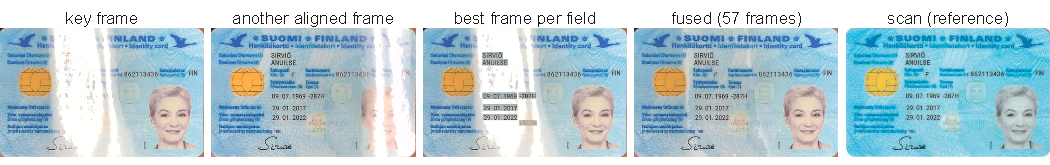
\includegraphics[width=\textwidth]{figures/fusion}
\caption{Fusion of a MIDV-2020 clip. Glare moves with the camera, the document does not.}
\label{fig:fusion}
\end{figure*}

\textbf{The effect depends on the reader} (Table~\ref{tab:glare}, Fig.~\ref{fig:halo}). Tesseract, which binarizes the line, reads 0.417 of the halo characters on our cards and 0.837 on the reference; the fine-tuned network recovers half of this gap (+0.216). PaddleOCR already reads 0.869 of the untreated halo, and every method lowers that: the processed strokes (Fig.~\ref{fig:glare}) confuse it more than the veil. Both signs of the networks repeat on 100 MIDV photos (fine-tuned: +0.125 and $-$0.086) and on the clips' key frames; the classical method is neutral on MIDV photos. Clipped text is not recovered by any single-image method.

\textbf{SSIM and OCR disagree.} On our test cards the fine-tuned network raises SSIM inside the glare from 0.511 to 0.624. The zero-shot network has the best whole-card SSIM (0.748, untreated 0.696), partly because it smooths the whole card, but it is the worst method for PaddleOCR in the halo.

\textbf{Do our modifications help?} (Table~\ref{tab:mod}.) Fine-tuning helps both networks on our cards: Restormer for Tesseract, DocSHRNet for both engines. But the gain of DocSHRNet over zero-shot is not significant on MIDV, where the glare is mostly textured reflection. Its detection head overfits (IoU with the glare mask 0.59 on train, 0.30 on test). The statistics veil helps Tesseract only, and the adaptive Wiener filter raises SSIM without raising accuracy. The classical method acts only near clipped seeds (76 of 94 images).

\begin{table*}[t]
\centering
\caption{Both artifacts: paired change of character accuracy (all boxes) vs untreated. A $\rightarrow$ B: A first. Both networks fine-tuned.}
\label{tab:joint}
\begin{tabular}{lllll}
\toprule
 & \multicolumn{2}{c}{blur + glare, our test ($n=9$)} & \multicolumn{2}{c}{glare, MIDV photos ($n=100$)} \\
\cmidrule(lr){2-3}\cmidrule(lr){4-5}
method & PaddleOCR & Tesseract & PaddleOCR & Tesseract \\
\midrule
untreated (accuracy) & .550 & .189 & .887 & .534 \\
\midrule
classical deglare & $-$.003 [$-$.011, .004] & \textbf{+.033 [.004, .067]} & \textbf{$-$.008 [$-$.016, $-$.002]} & +.000 [$-$.007, .007] \\
DL deglare & +.003 [$-$.010, .018] & \textbf{+.051 [.001, .130]} & \textbf{$-$.052 [$-$.067, $-$.040]} & \textbf{+.074 [.055, .094]} \\
Wiener, fixed & $-$.121 [$-$.305, .007] & $-$.061 [$-$.201, .064] & \textbf{$-$.465 [$-$.496, $-$.432]} & \textbf{$-$.476 [$-$.523, $-$.429]} \\
Wiener, adaptive & $-$.078 [$-$.259, .018] & $-$.013 [$-$.068, .043] & \textbf{$-$.046 [$-$.068, $-$.027]} & \textbf{$-$.058 [$-$.092, $-$.030]} \\
Restormer (ft) & \textbf{+.087 [.006, .175]} & \textbf{+.294 [.169, .426]} & \textbf{$-$.005 [$-$.008, $-$.001]} & \textbf{+.011 [.001, .023]} \\
Restormer $\rightarrow$ DL & \textbf{+.090 [.006, .179]} & \textbf{+.339 [.223, .454]} & \textbf{$-$.059 [$-$.077, $-$.043]} & \textbf{+.086 [.066, .107]} \\
DL $\rightarrow$ Restormer & \textbf{+.094 [.009, .186]} & \textbf{+.332 [.228, .433]} & \textbf{$-$.056 [$-$.071, $-$.042]} & \textbf{+.067 [.047, .087]} \\
\midrule
reference (accuracy) & .989 & .852 & .994 & .896 \\
\bottomrule
\end{tabular}

\end{table*}

\textbf{Several frames recover clipped text} (Table~\ref{tab:fusion}, Fig.~\ref{fig:fusion}). On keymax frames fusion raises core accuracy by 0.504 [0.459, 0.550] for PaddleOCR and 0.720 [0.670, 0.768] for Tesseract, close to the scan. In 99 of 100 clips every clipped core pixel is unclipped in another frame. Reading each field from its best frame achieves almost the same: over all fields fusion adds only 0.006 (PaddleOCR) and 0.013 (Tesseract) on keymax. The temporal median is worse in the core and overall: it also blurs clean text.

\subsection{Blur and glare together}
On our BG test images (Table~\ref{tab:joint}) the fine-tuned Restormer does most of the work: +0.087 for PaddleOCR and +0.294 for Tesseract. Adding DocSHRNet after it changes PaddleOCR by +0.003 [$-$0.015, 0.018] and Tesseract by +0.045 [0.008, 0.088]. The two orders do not differ significantly (Restormer first: $-$0.004 and +0.007). The best chain, Restormer $\rightarrow$ DocSHRNet, still leaves about 70\% of PaddleOCR's and 44\% of Tesseract's gap to the reference. On sharp glare photos Restormer does no harm (PaddleOCR +0.000, Tesseract +0.036). MIDV photos were chosen for glare, not blur; there Restormer is nearly neutral, and the chain inherits the engine-dependent effect of glare removal. Deblurring fused clips changes nothing (PaddleOCR +0.001, Tesseract +0.000 on keymax). Wiener hurts unblurred images.

\textbf{Runtime} per $1012\times638$ image on an M2 laptop: Wiener 0.05\,s, adaptive 2.7\,s, classical glare 0.09\,s (CPU); DocSHRNet 2.4\,s, Restormer 19.6\,s (GPU).

\section{Discussion and conclusion}
\label{sec:conclusion}
Restoration should be chosen together with the reader. For a binarizing engine, deblur with a fine-tuned network and then remove glare. A modern recognizer reads the halo without help and gains only from deblurring truly blurred images. Clipped text needs another frame: an app should capture a short burst and read each field from its best frame, and ask for a retake instead of inventing strokes. Generated digits are a real risk for ID data.

\textbf{Deviations from the proposal.} DocSHRNet replaces the unavailable network; the statistics veil replaces hysteresis with low-pass correction; the routing stage was dropped; fixed-box OCR replaces PSNR and LPIPS; Restormer was fine-tuned on real pairs only; MIDV photos replace our own hand-held set; and 14 of our 22 card sides are real, not mock.

\textbf{Limitations.} The test split has four cards and 4--9 images per condition. The noise floor is a proxy, since each card has one clean photo. The boxes come from PaddleOCR's detector. The networks saw 16 and 31 training photos. Unreported early blur pilots had seen test cards, so the choice of method families was not blind.

\textbf{Future work.} A per-field recapture flag, training on more cards, a second clean reference per card, and face verification.

\let\oldthebibliography\thebibliography
\renewcommand{\thebibliography}[1]{\oldthebibliography{#1}\setlength{\itemsep}{1pt}\setlength{\parsep}{0pt}}
\bibliographystyle{IEEEbib}
\bibliography{refs}
\end{document}
